\begin{frame}{Control supervisor: migración Stateflow → SFC}
  \centering
  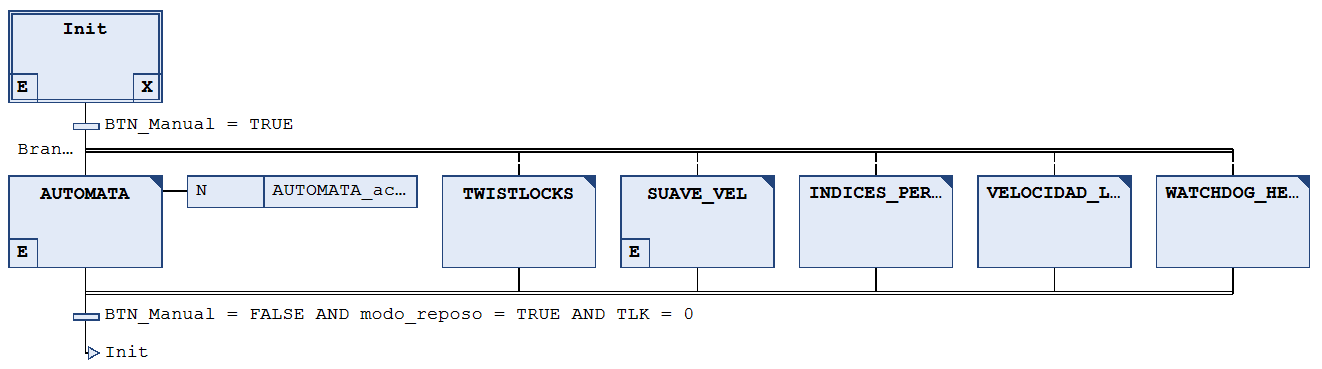
\includegraphics[width=0.95\textwidth]{codesys/codesys_supervisor11.png}
  
  Conversión de bloques Stateflow a SFC (Sequential Function Chart) manteniendo estados y transiciones
\end{frame}

\begin{frame}{Autómata principal en CODESYS}
  \centering
  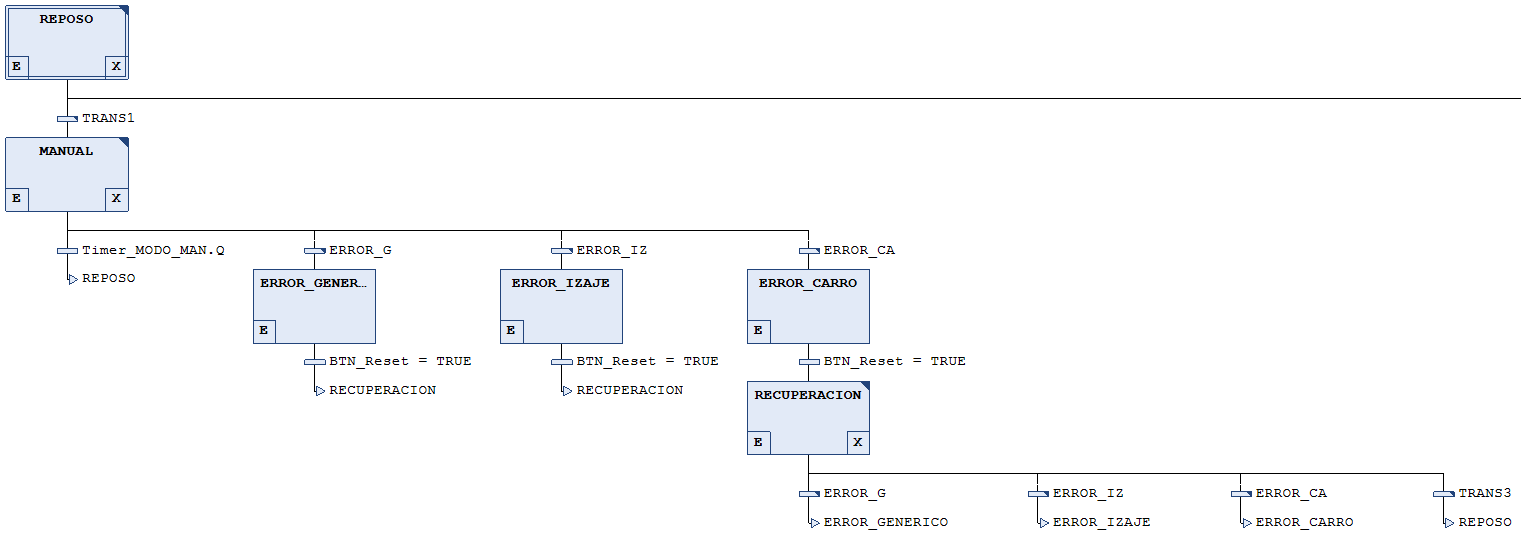
\includegraphics[width=0.95\textwidth]{codesys/codesys_supervisor12.png}
  
  \vspace{0.2cm}
  
  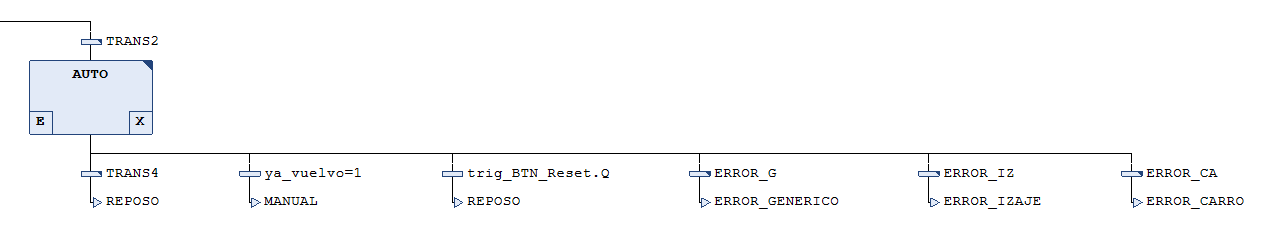
\includegraphics[width=0.95\textwidth]{codesys/codesys_supervisor13.png}
  
  Alternancia entre: REPOSO, MANUAL, AUTOMÁTICO, ERROR, RECUPERACIÓN
\end{frame}

\begin{frame}{Modo automático: adaptaciones de Stateflow a SFC}
  \centering
  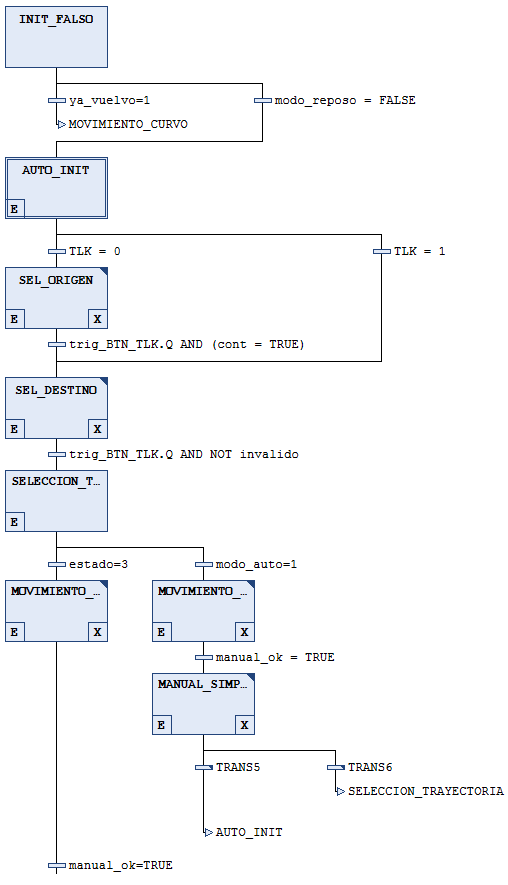
\includegraphics[width=0.7\textwidth]{codesys/codesys_supervisor15.png}
  
  Estado inicial vacío + transición FALSE para cumplir requisitos sintácticos de SFC
\end{frame}

\begin{frame}{Lógica de Twistlocks}
  \centering
  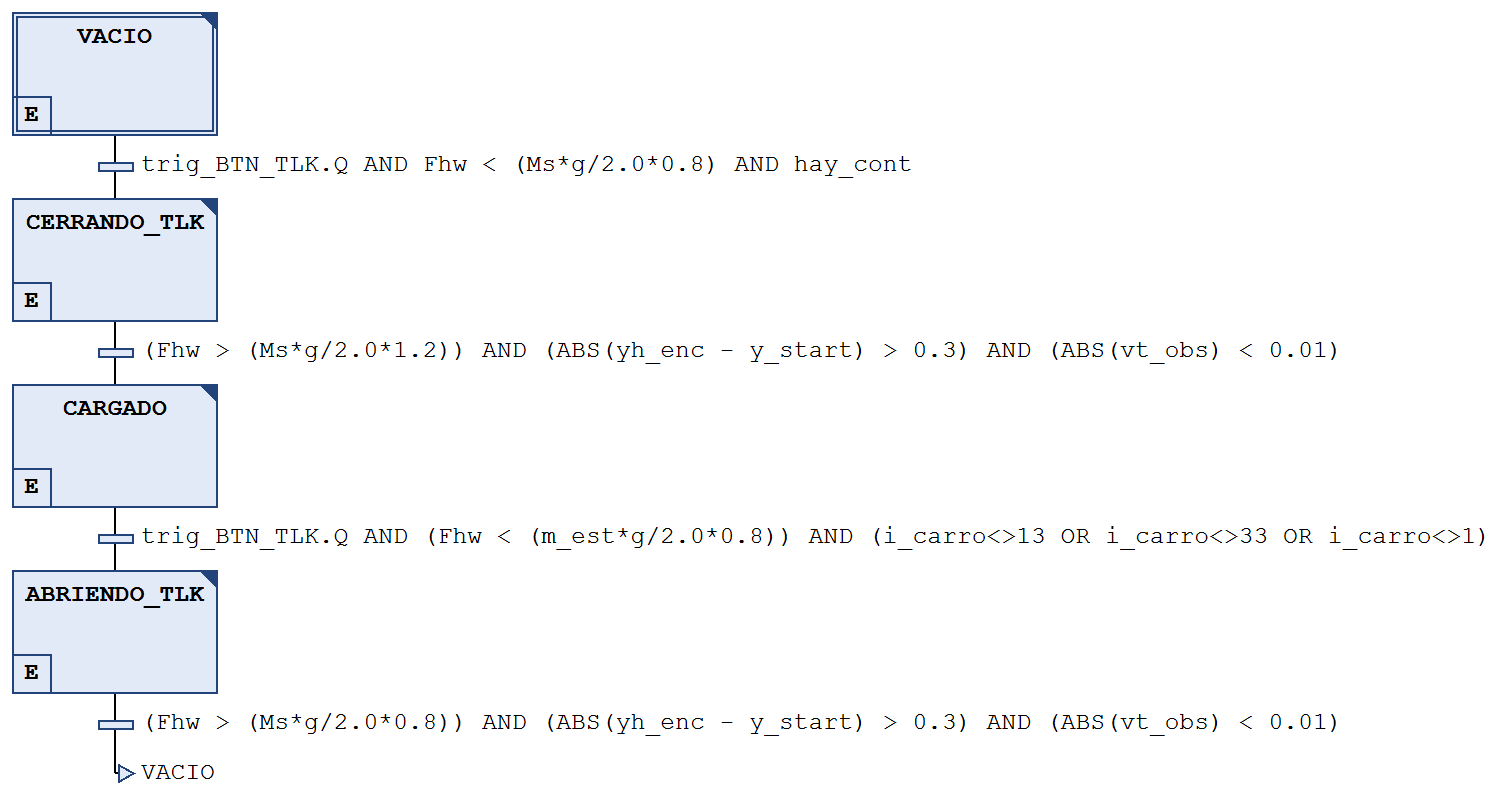
\includegraphics[width=0.85\textwidth]{codesys/codesys_supervisor4.png}
  
  SFC cíclico: últimos pasos retornan al estado inicial
\end{frame}

\begin{frame}{Cálculo de perfil e índices del muelle}
  \centering
  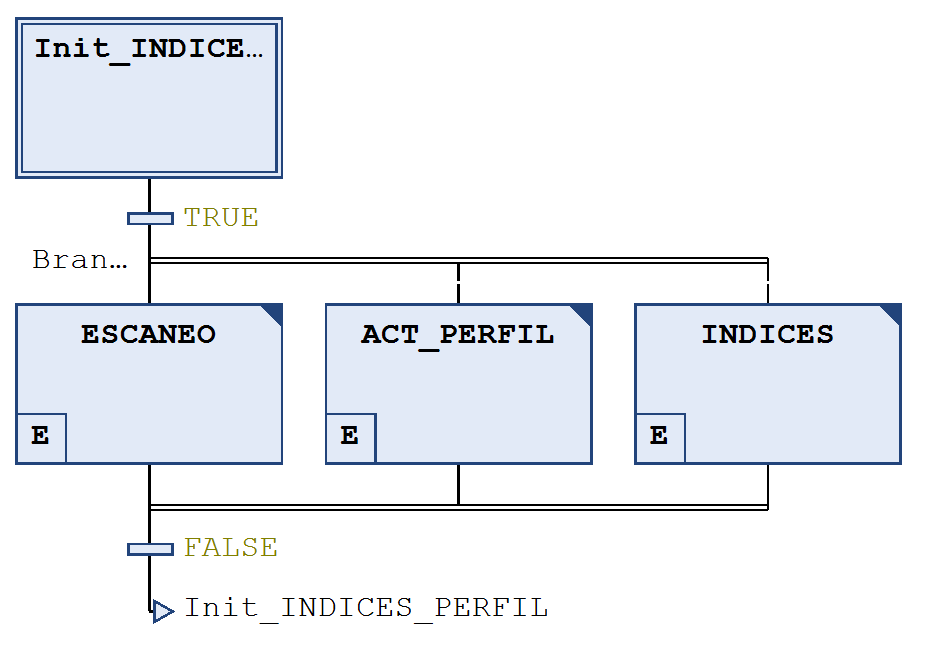
\includegraphics[width=0.8\textwidth]{codesys/codesys_supervisor14.png}
  
  Posición discreta del carro + actualización dinámica del perfil de obstáculos
\end{frame}

\begin{frame}{Bloques complementarios}
  \begin{block}{Suavizado de velocidad}
    Implementado en ST: suaviza referencias de velocidad
  \end{block}
  
  \begin{block}{Velocidad límites}
    Implementado en ST: aplicación de límites de velocidad por zona
  \end{block}
  
  \begin{block}{Watchdog heartbeat}
    Implementado en ST: monitoreo de comunicación con sistema de control
  \end{block}
\end{frame}

\subsection{Comunicación OPC-UA Simulink/CODESYS}

\begin{frame}{Protocolo OPC-UA para comunicación Simulink/CODESYS}
  \centering
  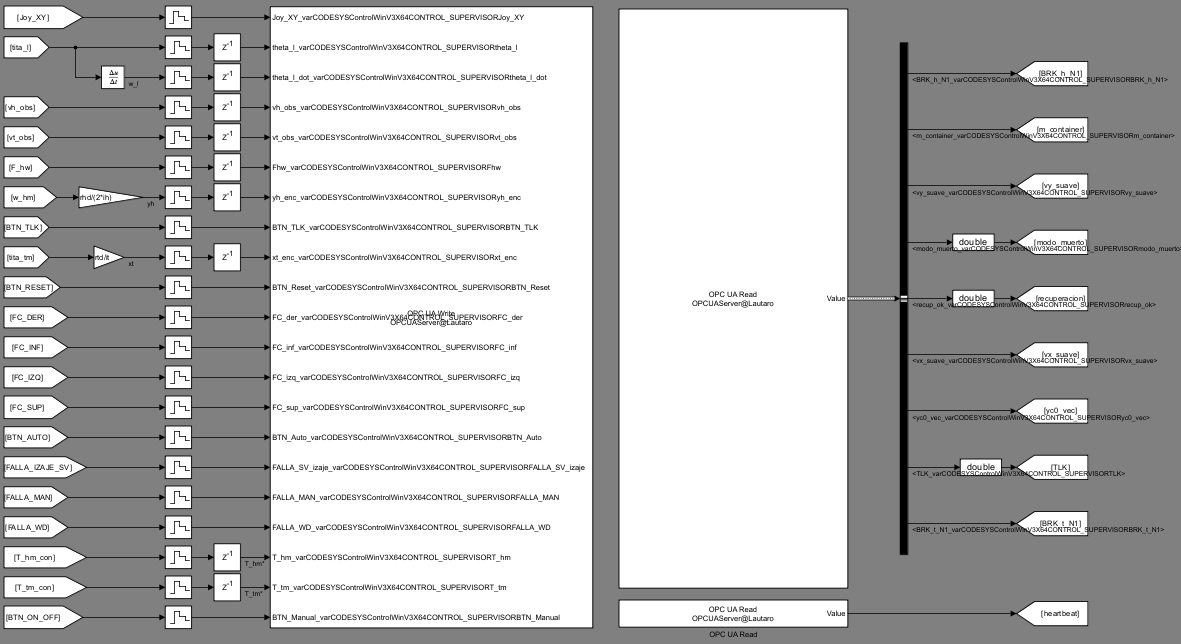
\includegraphics[width=0.85\textwidth]{codesys/opc_ua_1.png}
  
  Servidor OPC-UA en CODESYS con cliente en Matlab R2025b. Configuración: \textit{User allow anonymous} para lectura/escritura en tiempo real
\end{frame}

\begin{frame}{Bloques de comunicación: control de protección}
  \centering
  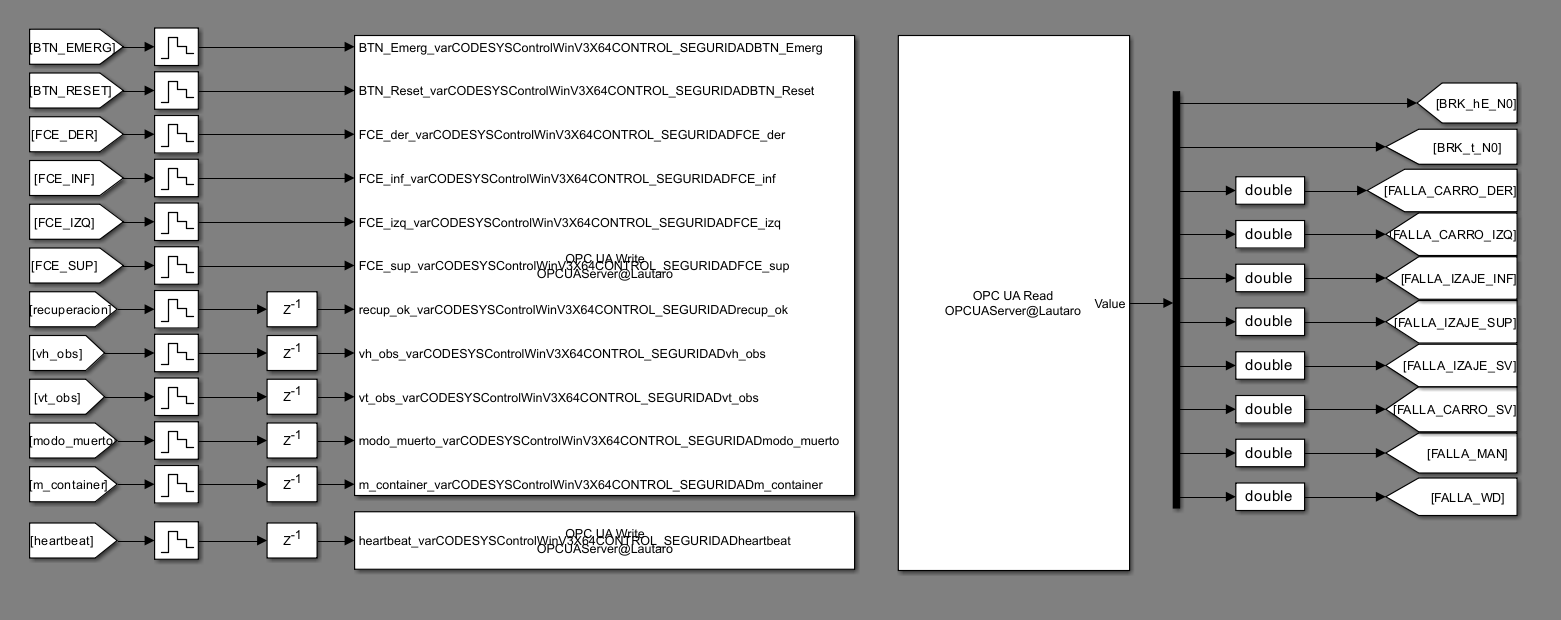
\includegraphics[width=0.9\textwidth]{codesys/opc_ua_0.png}
  
  Lectura/escritura de variables de protección (Nivel 0) a través de OPC-UA
\end{frame}

\begin{frame}{Desafío: retardo de comunicación}
  \begin{block}{Problema}
    OPC es protocolo TCP/IP diseñado para SCADA (retardos $\geq 500$ ms), no para control tiempo real
  \end{block}
  
  \begin{block}{Solución implementada}
    Bloques de comunicación con tiempos de muestreo diferenciados:
    \begin{itemize}
      \item Control supervisor y protección: $500$ ms
      \item Watchdog heartbeat: $20$ ms (tiempo original)
    \end{itemize}
    Reduce carga en red permitiendo Simulink correr a $1$s por segundo de simulación
  \end{block}
\end{frame}

\begin{frame}{Simulación con OPC-UA en funcionamiento}
  \centering
  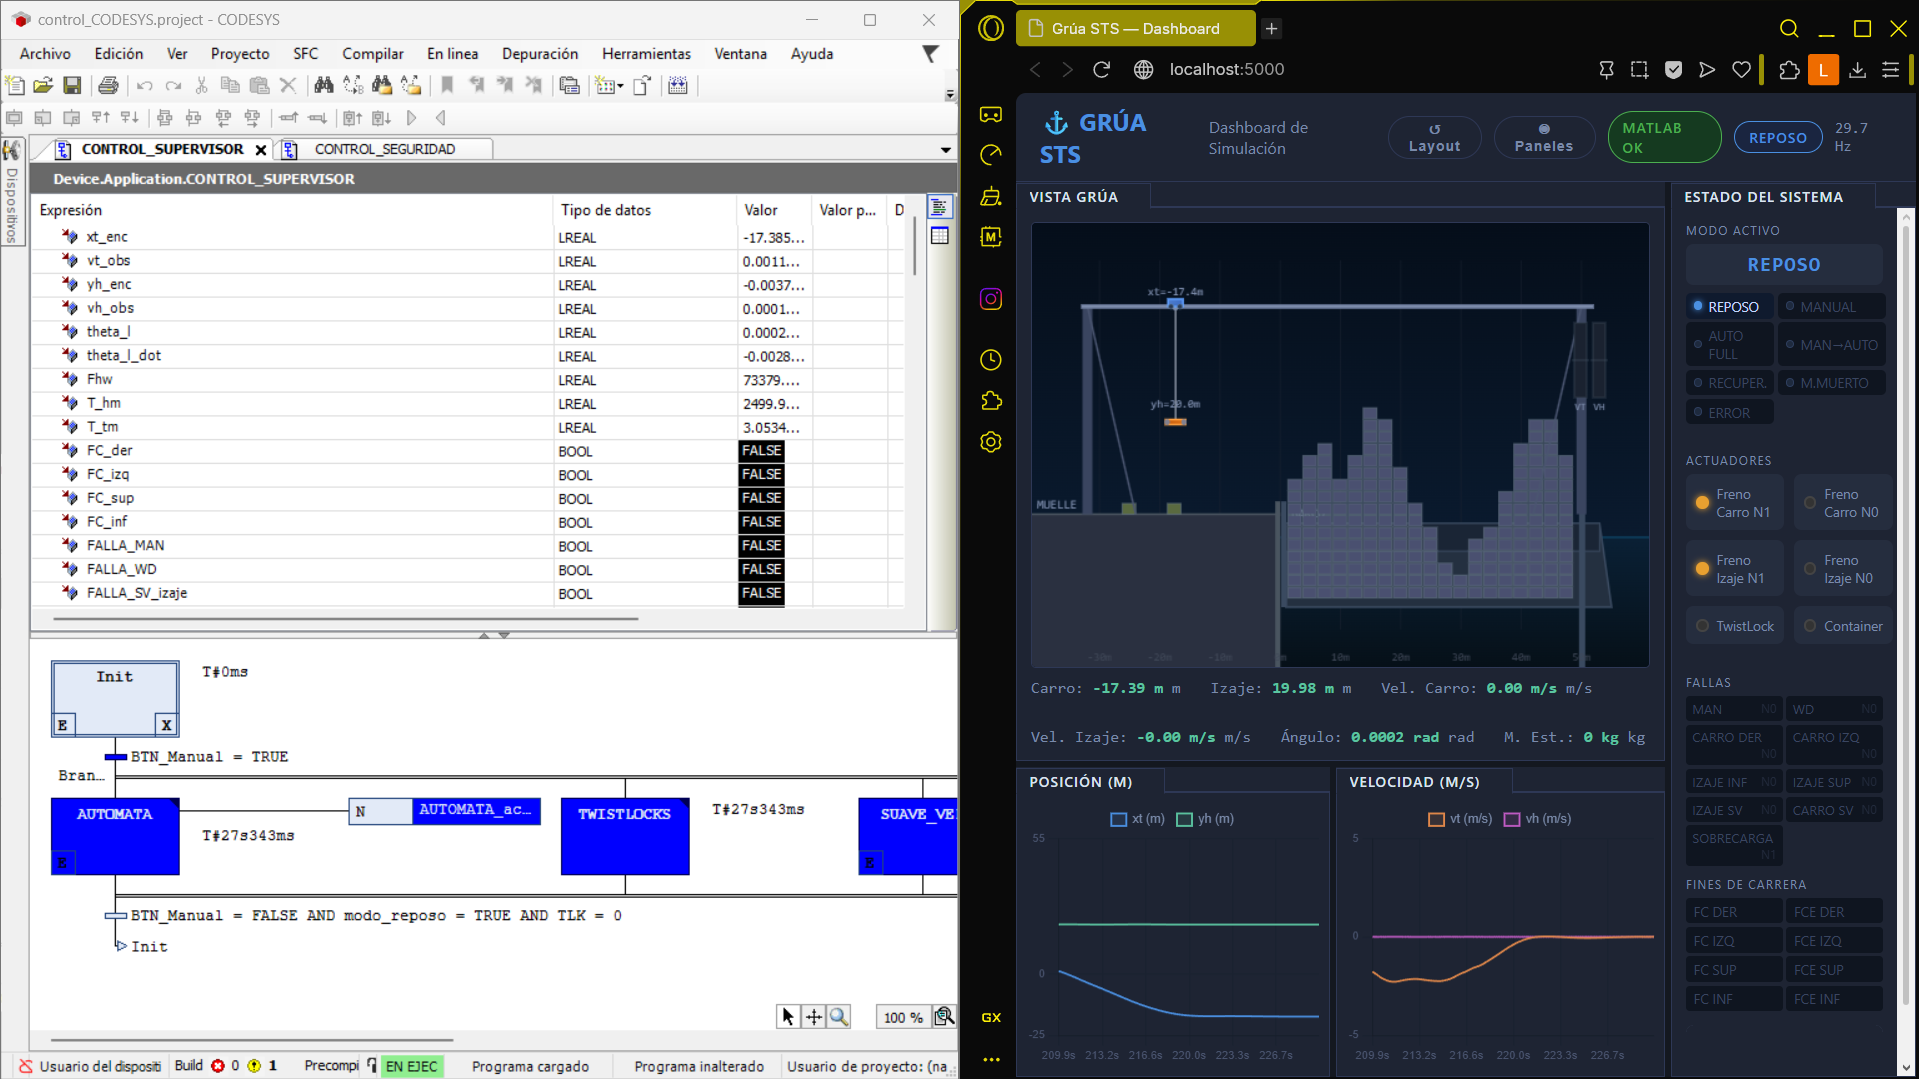
\includegraphics[width=0.9\textwidth]{codesys/codesys_interfaz.png}
  
  Mejora significativa en fluidez de simulación con comunicación OPC-UA. Controlador responde de forma equivalente al modelo en Simulink
\end{frame}

